\pdfminorversion=4
\documentclass[aspectratio=169]{beamer}

\mode<presentation>
{
  \usetheme{default}
  \usecolortheme{default}
  \usefonttheme{default}
  \setbeamertemplate{navigation symbols}{}
  \setbeamertemplate{caption}[numbered]
  \setbeamertemplate{footline}[frame number]  % or "page number"
  \setbeamercolor{frametitle}{fg=white}
  \setbeamercolor{footline}{fg=black}
} 

\usepackage[english]{babel}
\usepackage[utf8x]{inputenc}
\usepackage{tikz}
\usepackage{courier}
\usepackage{array}
\usepackage{bold-extra}
\usepackage{minted}
\usepackage[thicklines]{cancel}
\usepackage{fancyvrb}

\xdefinecolor{dianablue}{rgb}{0.18,0.24,0.31}
\xdefinecolor{darkblue}{rgb}{0.1,0.1,0.7}
\xdefinecolor{darkgreen}{rgb}{0,0.5,0}
\xdefinecolor{darkgrey}{rgb}{0.35,0.35,0.35}
\xdefinecolor{darkorange}{rgb}{0.8,0.5,0}
\xdefinecolor{darkred}{rgb}{0.7,0,0}
\definecolor{darkgreen}{rgb}{0,0.6,0}
\definecolor{mauve}{rgb}{0.58,0,0.82}

\title[2020-10-26-as-blueprint-uproot-awkward]{Access and manipulation of complex data structures: \\ Uproot and Awkward Array}
\author{Jim Pivarski}
\institute{Princeton University -- IRIS-HEP}
\date{October 26, 2020}

\usetikzlibrary{shapes.callouts}

\begin{document}

\logo{\pgfputat{\pgfxy(0.11, 7.4)}{\pgfbox[right,base]{\tikz{\filldraw[fill=dianablue, draw=none] (0 cm, 0 cm) rectangle (50 cm, 1 cm);}\mbox{\hspace{-8 cm}\includegraphics[height=1 cm]{princeton-logo-long.png}\hspace{0.1 cm}\raisebox{0.1 cm}{\includegraphics[height=0.8 cm]{iris-hep-logo-long.png}}\hspace{0.1 cm}}}}}

\begin{frame}
  \titlepage
\end{frame}

\logo{\pgfputat{\pgfxy(0.11, 7.4)}{\pgfbox[right,base]{\tikz{\filldraw[fill=dianablue, draw=none] (0 cm, 0 cm) rectangle (50 cm, 1 cm);}\mbox{\hspace{-8 cm}\includegraphics[height=1 cm]{princeton-logo.png}\hspace{0.1 cm}\raisebox{0.1 cm}{\includegraphics[height=0.8 cm]{iris-hep-logo.png}}\hspace{0.1 cm}}}}}

% Uncomment these lines for an automatically generated outline.
%\begin{frame}{Outline}
%  \tableofcontents
%\end{frame}

% START START START START START START START START START START START START START

%% So I imagine each talk is
%% 1-2 slides: What is my project and why do I think it is important functionality for users? What functionality does it provide that either is not available elsewhere or is more performant than others?
%% 1-2 slide: What is the general status of my projects development and deployment?
%% 1-2 slides: What does my implementation look like to users? (API)
%% 1-2 slides: Where does my project fit into the overall context of End-to-End Analysis (@Kyle’s presentation)? Which other tools does my tool interface with and why are those interfaces likely to be?

%% One nugget from the other post: Please appreciate that there are people attending that are not in our close circle on this stuff and will be completely unable to understand and contribute if we just plow right into the details. That’s why I am stressing for the talks to have a slide or two on what the project is and what it provides for users. This is also why I’m against earlier suggestions of starting out the workshop with a panel of experts talking thorugh stuff. Thats the afternoon session and we have (at least) two hours to do that and achieve the Day 1 goes of (1) identifying useful and viable analysis system sets and (2) working through the interfaces between tools to realize a full analysis pipeline (edited)

\begin{frame}{Uproot \& Awkward Array: part of this complete analysis}
\vspace{0.17 cm}
\begin{columns}
\column{1.15\linewidth}
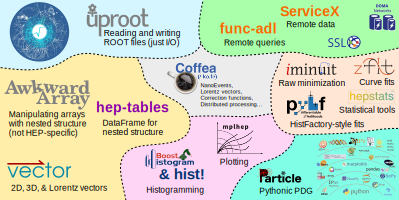
\includegraphics[width=\linewidth]{part-of-this-complete.pdf}
\end{columns}
\end{frame}

\end{document}
